\section*{EXAMPLES}
In this section, three different examples are discussed. Their purpose is to numerically showcase that our method allows to adaptively refine the mesh to accurately solve an OCP, similarly to ~\cite{Patterson:OCAM:2015}, with the remarkable advantage of an increased computational efficiency for the final enhanced mesh without hindering the accuracy of the final solution.
%still within the specified tolerance.
In fact, by allowing to increase the degrees of the approximating polynomials independently for each state, our method effectively adopts to raise them carefully and in a tailored manner. This allows to reduce the overall number of variables of the resulting NLP, with clear benefits in terms of reduced CPU time, memory usage and reduced risk of being trapped by local minima.

Let us now direct our attention to the details. Each problem is transcribed in its initial NLP version by choosing $N = 20$ mesh intervals and by assigning a degree $\dki = 2$ everywhere, i.e. for all $i = 1, \dots, n_x$ and  $k = 1, \dots, N$. The mesh refinement algorithm is then applied with $d_{\min} = 2$, $d_{\max} = 8$ with a prescribed maximum allowable relative error $\epsilon = 1 \cdot 10^{-3}$.

It is worth observing that the $p_{n}h$ and $ph$ tags indicate our mesh refinement method and the one originally proposed by Patterson et al.~\cite{Patterson:OCAM:2015}, respectively.

It is also worth remarking that the final refined mesh for all the three presented examples (both in terms of number and size of $S_{k}$ intervals), turns out to be the same by rolling out both the $p_{n}h$ and the $ph$ approaches. This arises partly as a result that both algorithms share the last section (lines 9-14) of the \emph{Execution} pass in {\bf Algorithm~\ref{alg:step2}}. This means the generic $S_k$ interval is subdivided if and only if at least one state in the generic $S_k$ asks for it.

Each transcribed optimal control problem tested was coded in a scripting environment using the \text{MATLAB} interface to the open-source CasADi framework~\cite{casadi:MPC:2019}.
The CasADi suite can perform AD (Automatic Differentiation) on the code to compute gradients and Jacobians and provides building blocks to efficiently formulate and solve large-scale optimization problems. The back-end solver adopted is IPOPT~\cite{Biegler:CCE:2009} which implements an interior-point algorithm. All the associated NLPs are solved on a laptop with 2.30GHz Intel(R) Core(TM) i7-10875H CPU and 32 GB of RAM.



%%%%%%%%%%%%%%%%%%%%%%%%%%%%%%%%%%%%%%%%%%%%%%%%%%%%%%%%%%%%%%%%%%%%%%
\subsection*{Example 1: Van Der Pol}
The first optimal control problem considered is taken from reference~\cite{casadi:DOC:2018} and considers
driving a \emph{Van der Pol} oscillator to the origin. It can be expressed as follows
\begin{subequations}\label{eq:vanderpol}
	\begin{align}
	\underset{X \in \mathbb{R}^{2}, \, U \in \mathbb{R}}{\text{minimize}}\hspace{8mm}
	&J = \int_{0}^{T}(x_1^{2} + x_2^{2} + u^{2})\,dt  \label{eq:vancost}\\
	\text{subject to} \hspace{8mm}
	& \dot{x}_1 = (1 - x_2^{2})x_{1} - x_2 + u \hspace{5mm} t \in[0,T] \label{eq:vandyn1}\\
	& \dot{x}_2 = x_1 \hspace{28.5mm} t \in[0,T] \label{eq:vandyn2}\\
	& -1  \leq u \leq 1,  \hspace{20mm} t \in[0,T] \label{eq:vanpath1}\\
	& x_2 \geq -0.25,  \hspace{21.5mm} t \in[0,T] \label{eq:vanpath2}\\
	 x_1(0) &= 0, \hspace{2mm} x_2(0) = 1, \label{eq:initial1}		
	%& x_2(0) = 1, \label{eq:intial2}		
	\end{align}
\end{subequations}
where $T = 10$ s, $x_1$ and $x_2$ are the two state components (hence $X(t) = [x_1(t), x_2(t)]\in \bbR^2$), $u\in\bbR$ indicates the control, and the dynamics constraints and the initial conditions are shown explicitly for each state component. Clearly, $\dot{X}(t) = [\dot{x}_1(t), \dot{x}_2(t)]$.

In Figs.~\ref{fig:pnh1vanderpol}-\ref{fig:pnh2vanderpol} (top panels) the final degrees of the first ($x_1$) and the second ($x_2$) state components, respectively, are shown. Here, the blue line is the outcome of the $\pnh$-mesh refinement algorithm whereas the green line is the result of the $ph$-one. With respect to the red line, which represents the initial degree, each method increases the degrees of the polynomials approximating the states. Is is worth noting that the green line is the same for both figures, meaning that, according to the $pn$ logic, all the states share the same (maximum) polynomial order in the same interval $S_k$. Instead, the blue lines are different, meaning that each state has reached an independent degree for its polynomial approximation.
Furthermore, with respect to the initial $S_k$ steps delimited by the dashed gray lines, the more packed green and blue markers of the final solutions reveal where the $h$-strategy was adopted, thus producing a finer mesh.

In Figs.~\ref{fig:pnh1vanderpol}-\ref{fig:pnh2vanderpol} (bottom panels) the state profiles obtained with the $\pnh$ final mesh are shown. Here, the dashed gray lines delimit the \emph{final} mesh intervals. In particular, the nodal values are shown in blue, whereas the collocation points are plotted in red. These figures clearly show that the $\pnh$-adaptive mesh refinement method increases the polynomial order (more collocation points) and increases the mesh density (more mesh points) selectively for each state only where it is needed (higher gradient).
\begin{figure}[t]
	\centering
	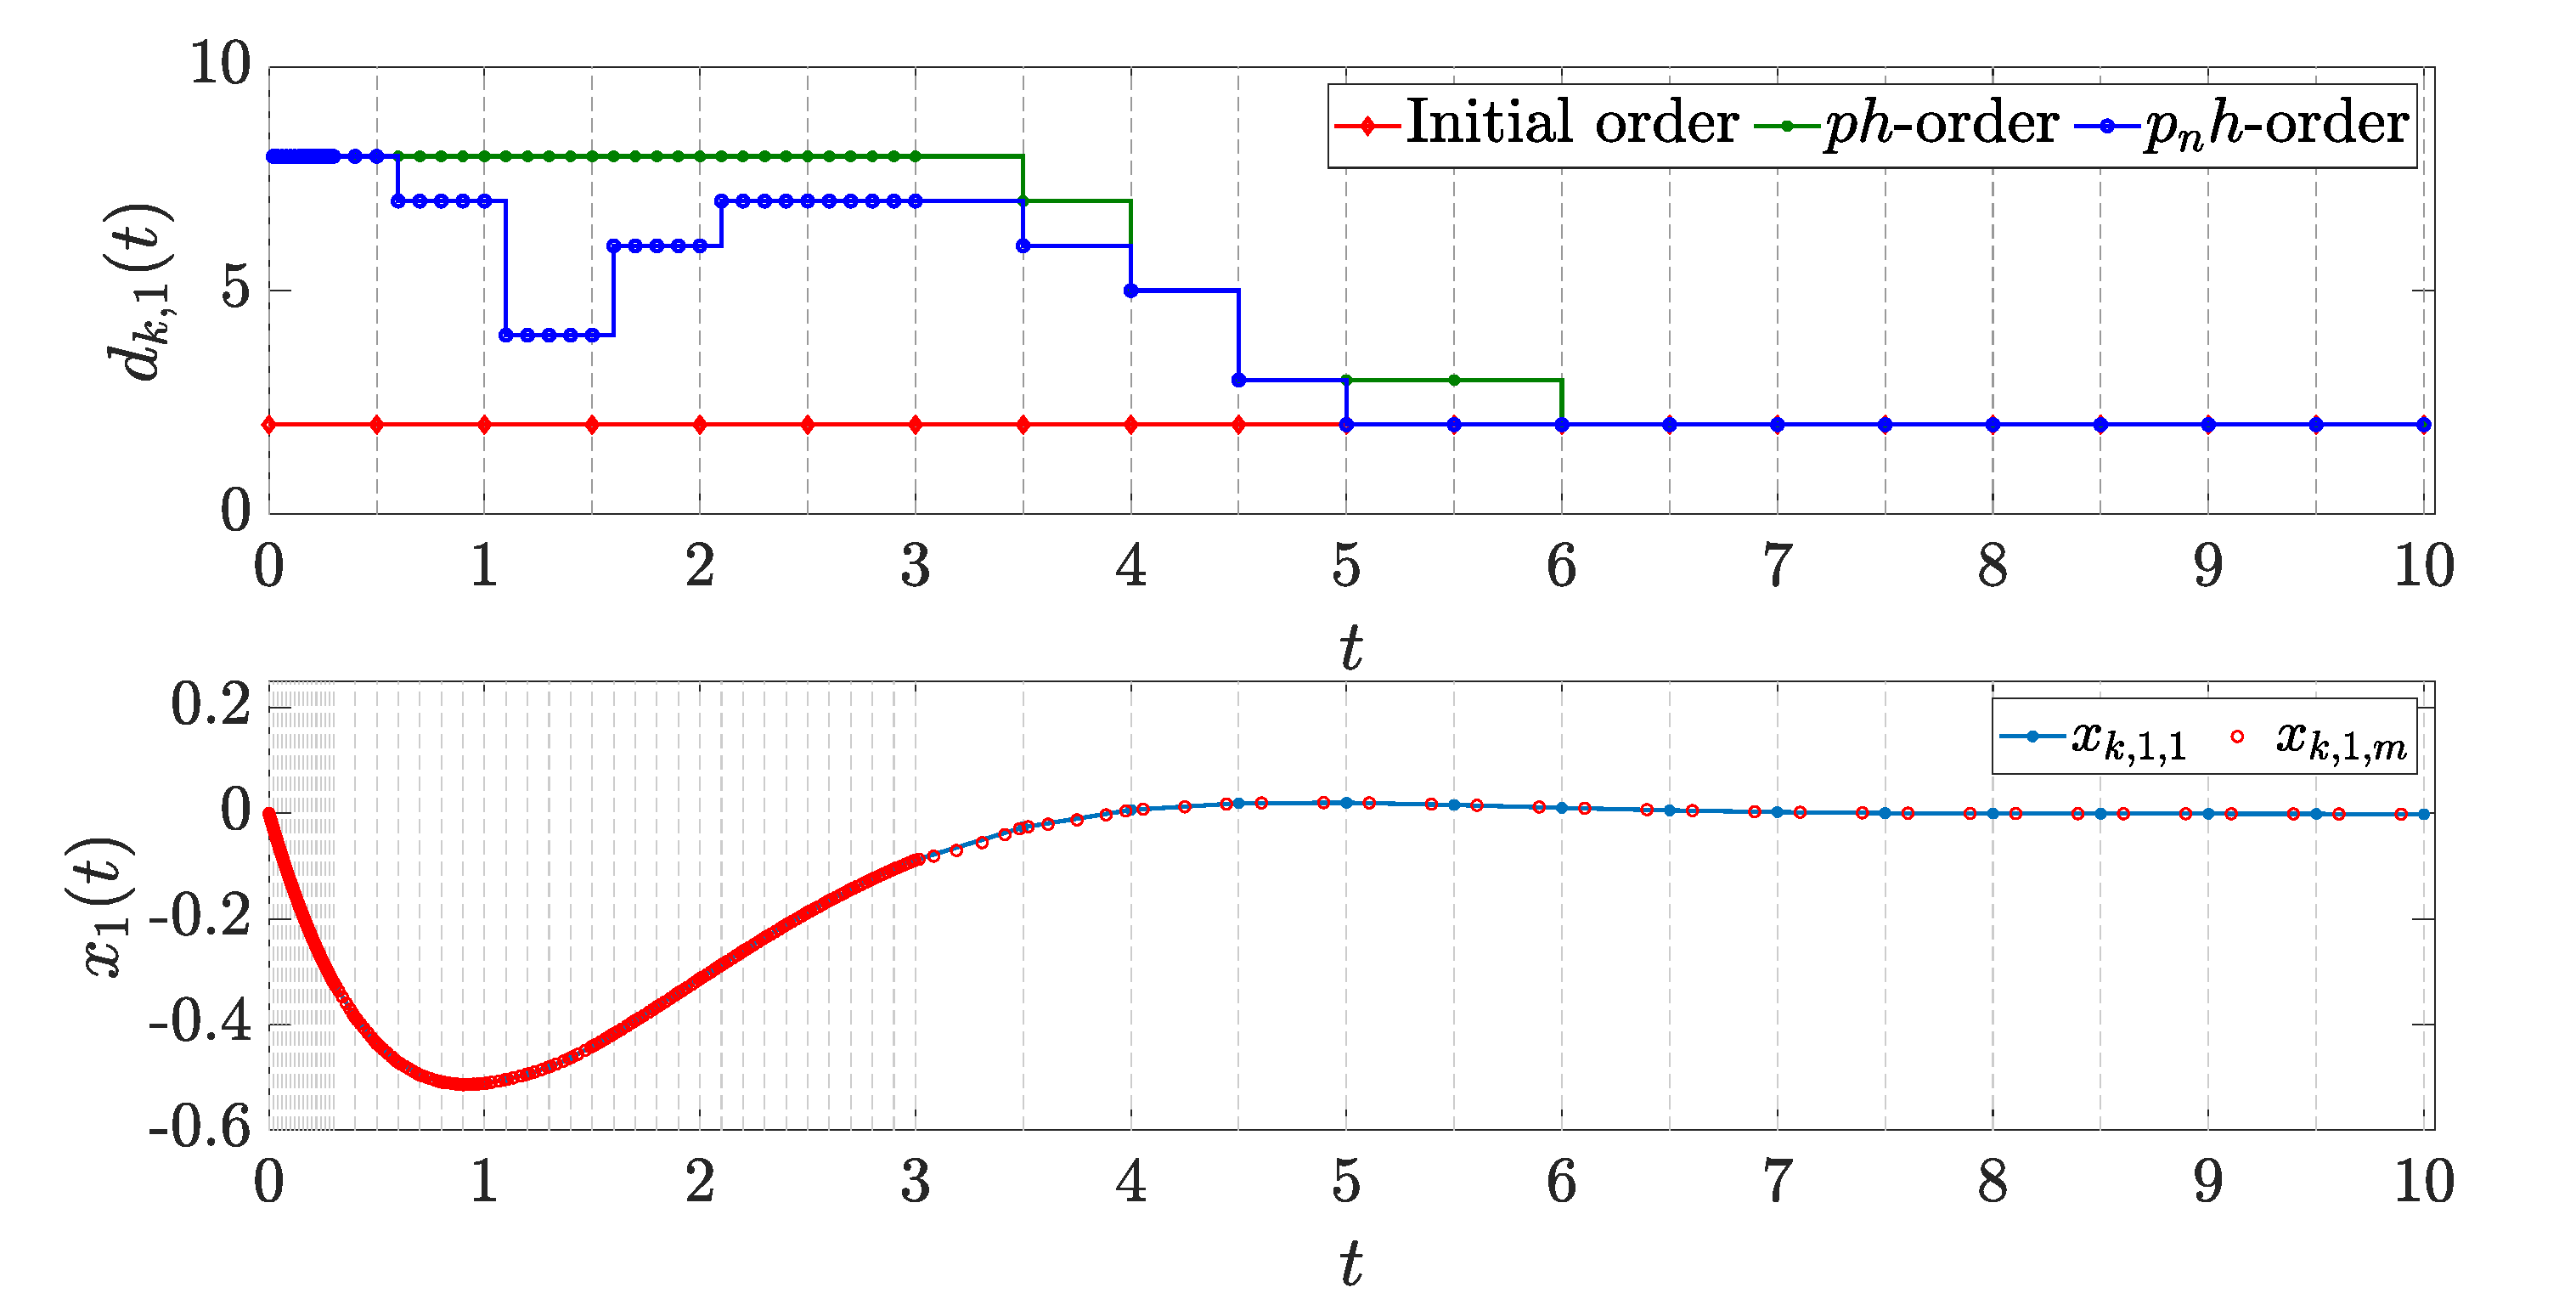
\includegraphics[trim={1cm 0.1cm 2cm 0.5cm},clip,width=1\columnwidth]{Img/pnh1_vanderpol1}
	\caption{EXAMPLE 1:  (TOP) POLYNOMIAL DEGREE OF $x_{1}$ FOR THE INITIAL MESH (RED) FOR $\pnh$ ALGORITHM (BLUE) AND FOR $ph$ ALGORITHM (GREEN), (BOTTOM)
	OPTIMAL $x_1$ PROFILE OBTAINED WITH $\pnh$.}
	\label{fig:pnh1vanderpol}
\end{figure}
\begin{figure}[t]
	\centering
	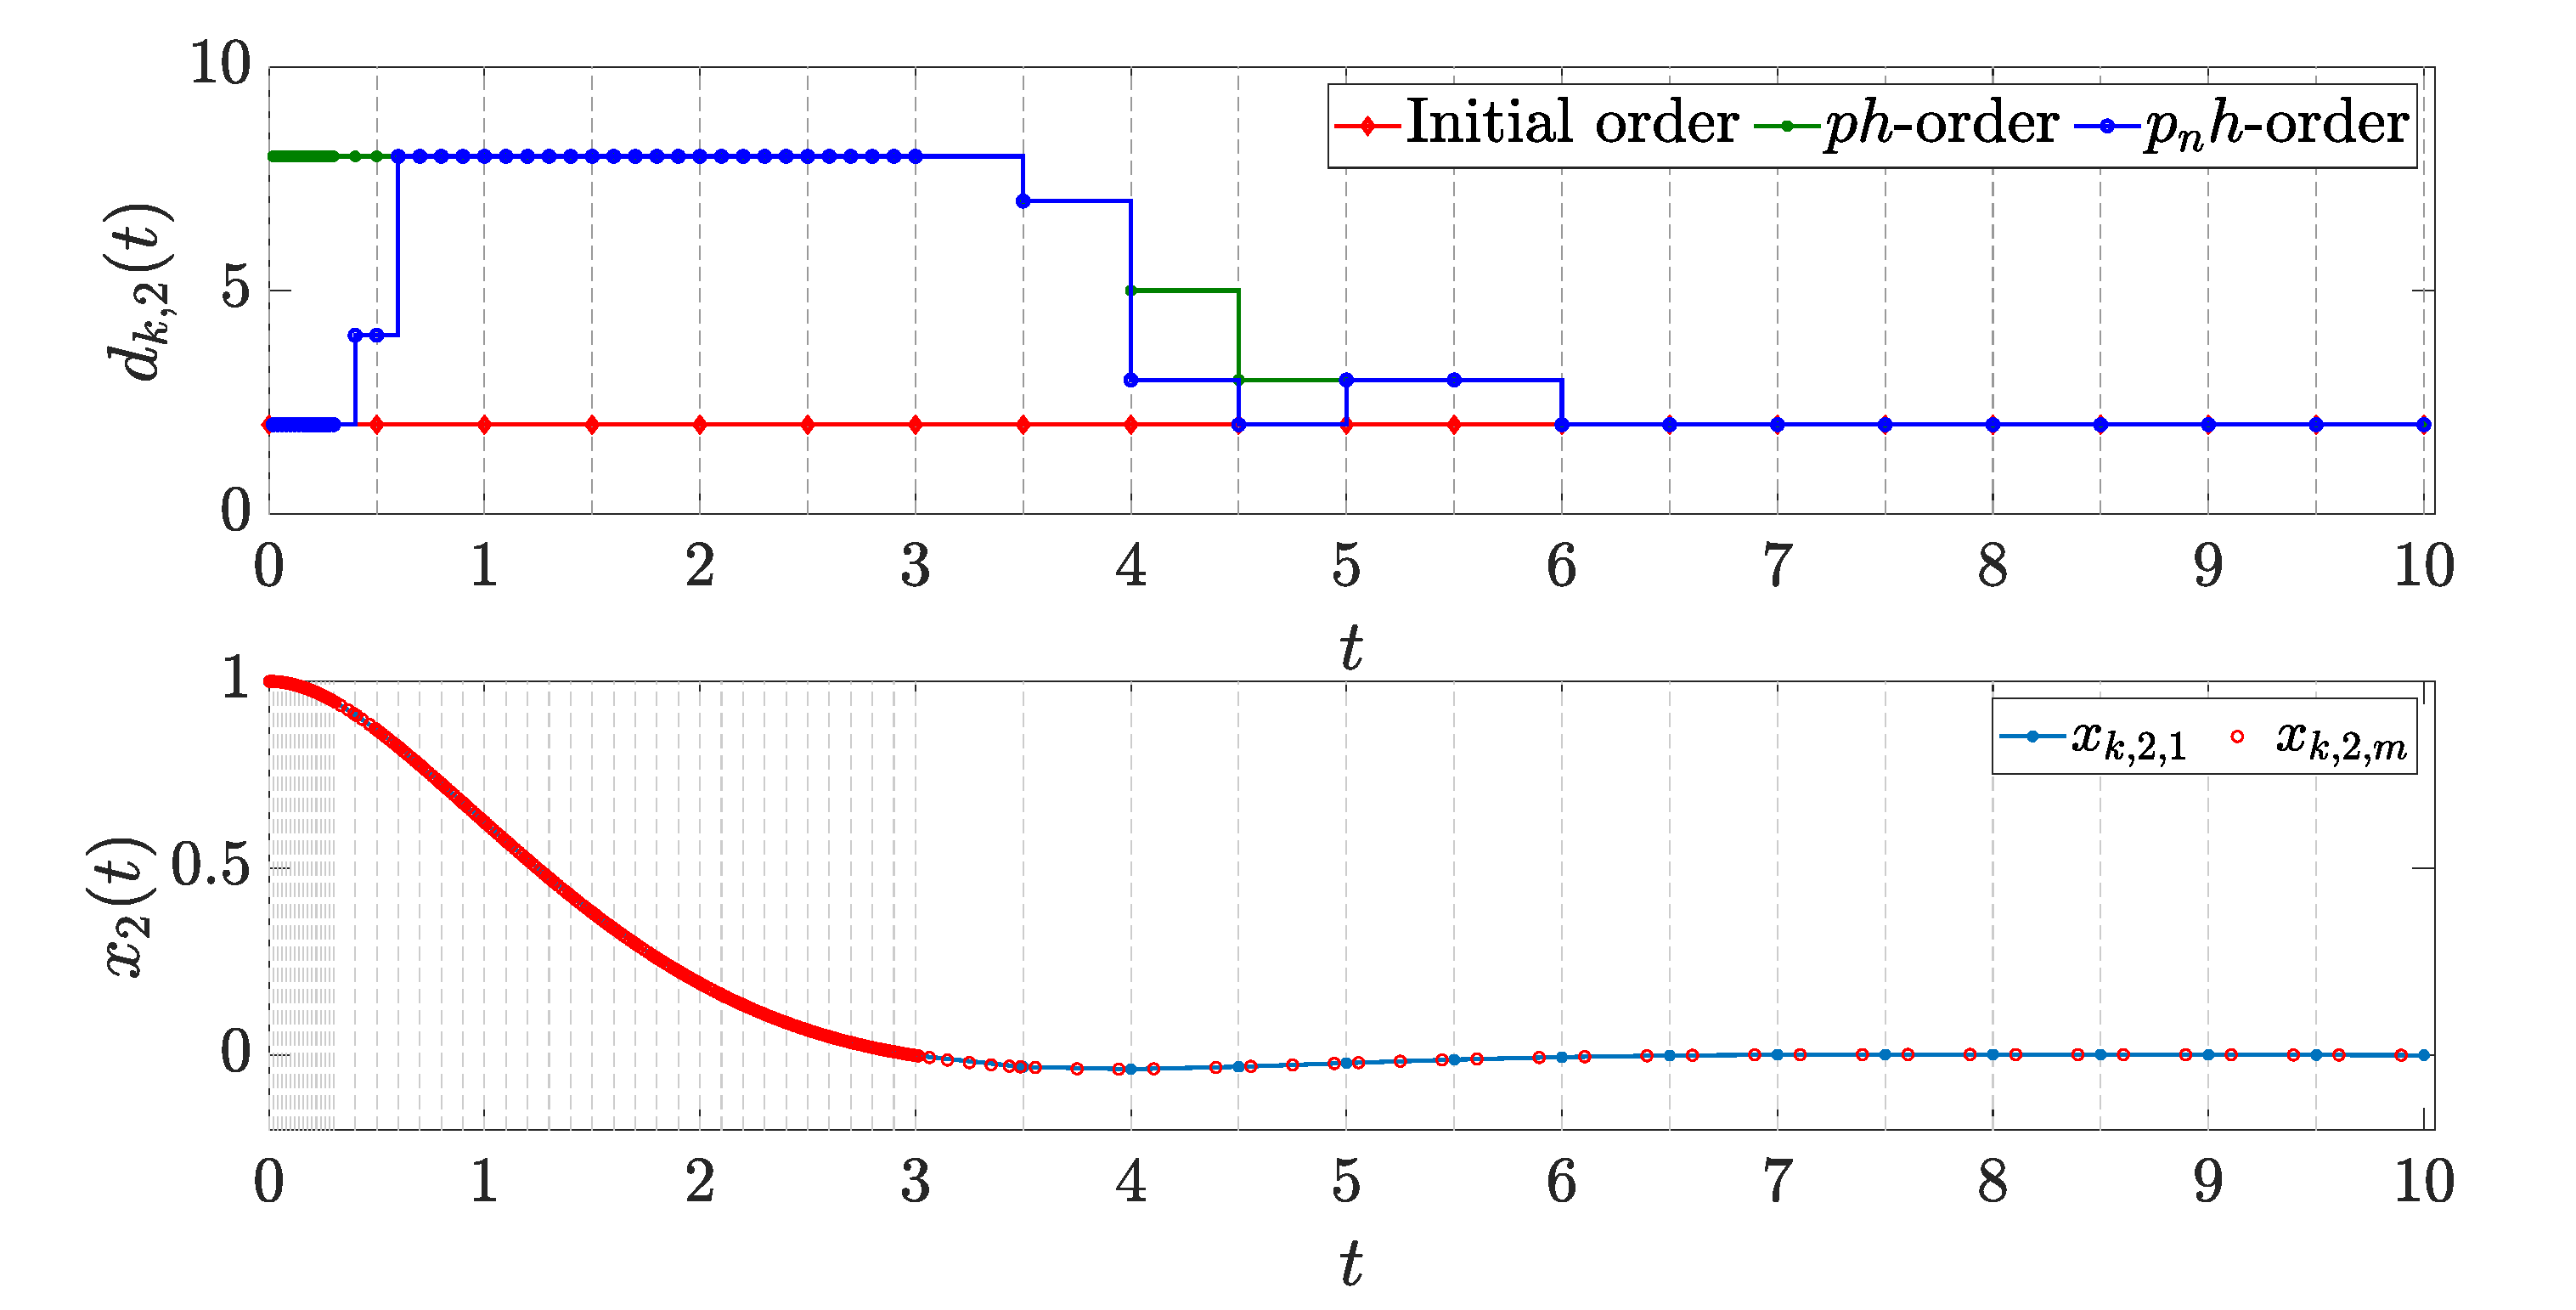
\includegraphics[trim={1cm 0.1cm 2cm 0.5cm},clip,width=1\columnwidth]{Img/pnh2_vanderpol2}
	\caption{EXAMPLE 1: (TOP) POLYNOMIAL DEGREE OF $x_{2}$ FOR THE INITIAL MESH (RED) FOR $\pnh$ ALGORITHM (BLUE) AND FOR $ph$ ALGORITHM (GREEN) (TOP), (BOTTOM)
	OPTIMAL $x_1$ PROFILE OBTAINED WITH  $\pnh$.}
	\label{fig:pnh2vanderpol}
\end{figure}
The advantages of the $\pnh$ method with respect to the $ph$ one are shown in Table~\ref{tab:tablevanderpol}. Here, the \emph{Mesh} column indicates the type of discretization mesh. In particular, \emph{Initial} refers to the mesh of the initial problem, whereas $ph$ and $\pnh$ refer to the final meshes produced by applying the methods in~\cite{Patterson:OCAM:2015} and ours, respectively. Is is worth remarking that both of them comply with the prescribed tolerance $\epsilon=10^{-3}$. Furthermore, \emph{Vars} indicates the number of variables of the NLP associated to the transcribed OCP. Then, \emph{Soln. time} indicates the time to solution of the optimal control problem with the refined mesh. Finally, \emph{Iter} refers to the number of algorithm iterations needed to reach the prescribed accuracy, whereas \emph{Tot.\,time} is the total CPU time elapsed to reach the imposed convergence criterion. It is worth remarking that it includes the necessary time to build and solve all the \emph{Iter} $+1$ successive NLP problems and the time spent by the application of \emph{Iter} mesh refinement algorithms. Finally, $e_\text{max}$  is the maximum of the local error $\ekij$, hence
\begin{equation}
e_\text{max}= \max\limits_{\substack{j = 1, \dots, \dkip \\ i = 1, \dots, n_x \\ k = 1, \dots, N}} (\ekij)
\end{equation}
\begin{table}[t]
	\caption{EXAMPLE 1: MESH REFINEMENT RESULTS FOR THE THREE DIFFERENT TYPE OF MESH (INITIAL MESH, $ph$ FINAL MESH AND $\pnh$ FINAL MESH)}
	\begin{center}
		\label{tab:tablevanderpol}
		\begin{tabular}{c l l l c c c}
			& & \\ % put some space after the caption
			\hline
			\emph{Mesh} & \emph{Vars} & \emph{Soln. time} & \emph{Iter} & \emph{Tot. time} & $e_\text{max}$ \\
			\hline
			\emph{Initial} & 140 & 138ms & / & / &  $3.7\mathrm{e}{-2}$\\
			$ph$ & 918 & 500ms & 4 & 23.1s & $9.1\mathrm{e}{-4}$ \\
			$\pnh$ & 769 & 400ms & 4 & 19s & $9.5\mathrm{e}{-4}$ \\
			\hline
		\end{tabular}
	\end{center}
\end{table}
%%%%
\begin{figure}[t]
	\centering
	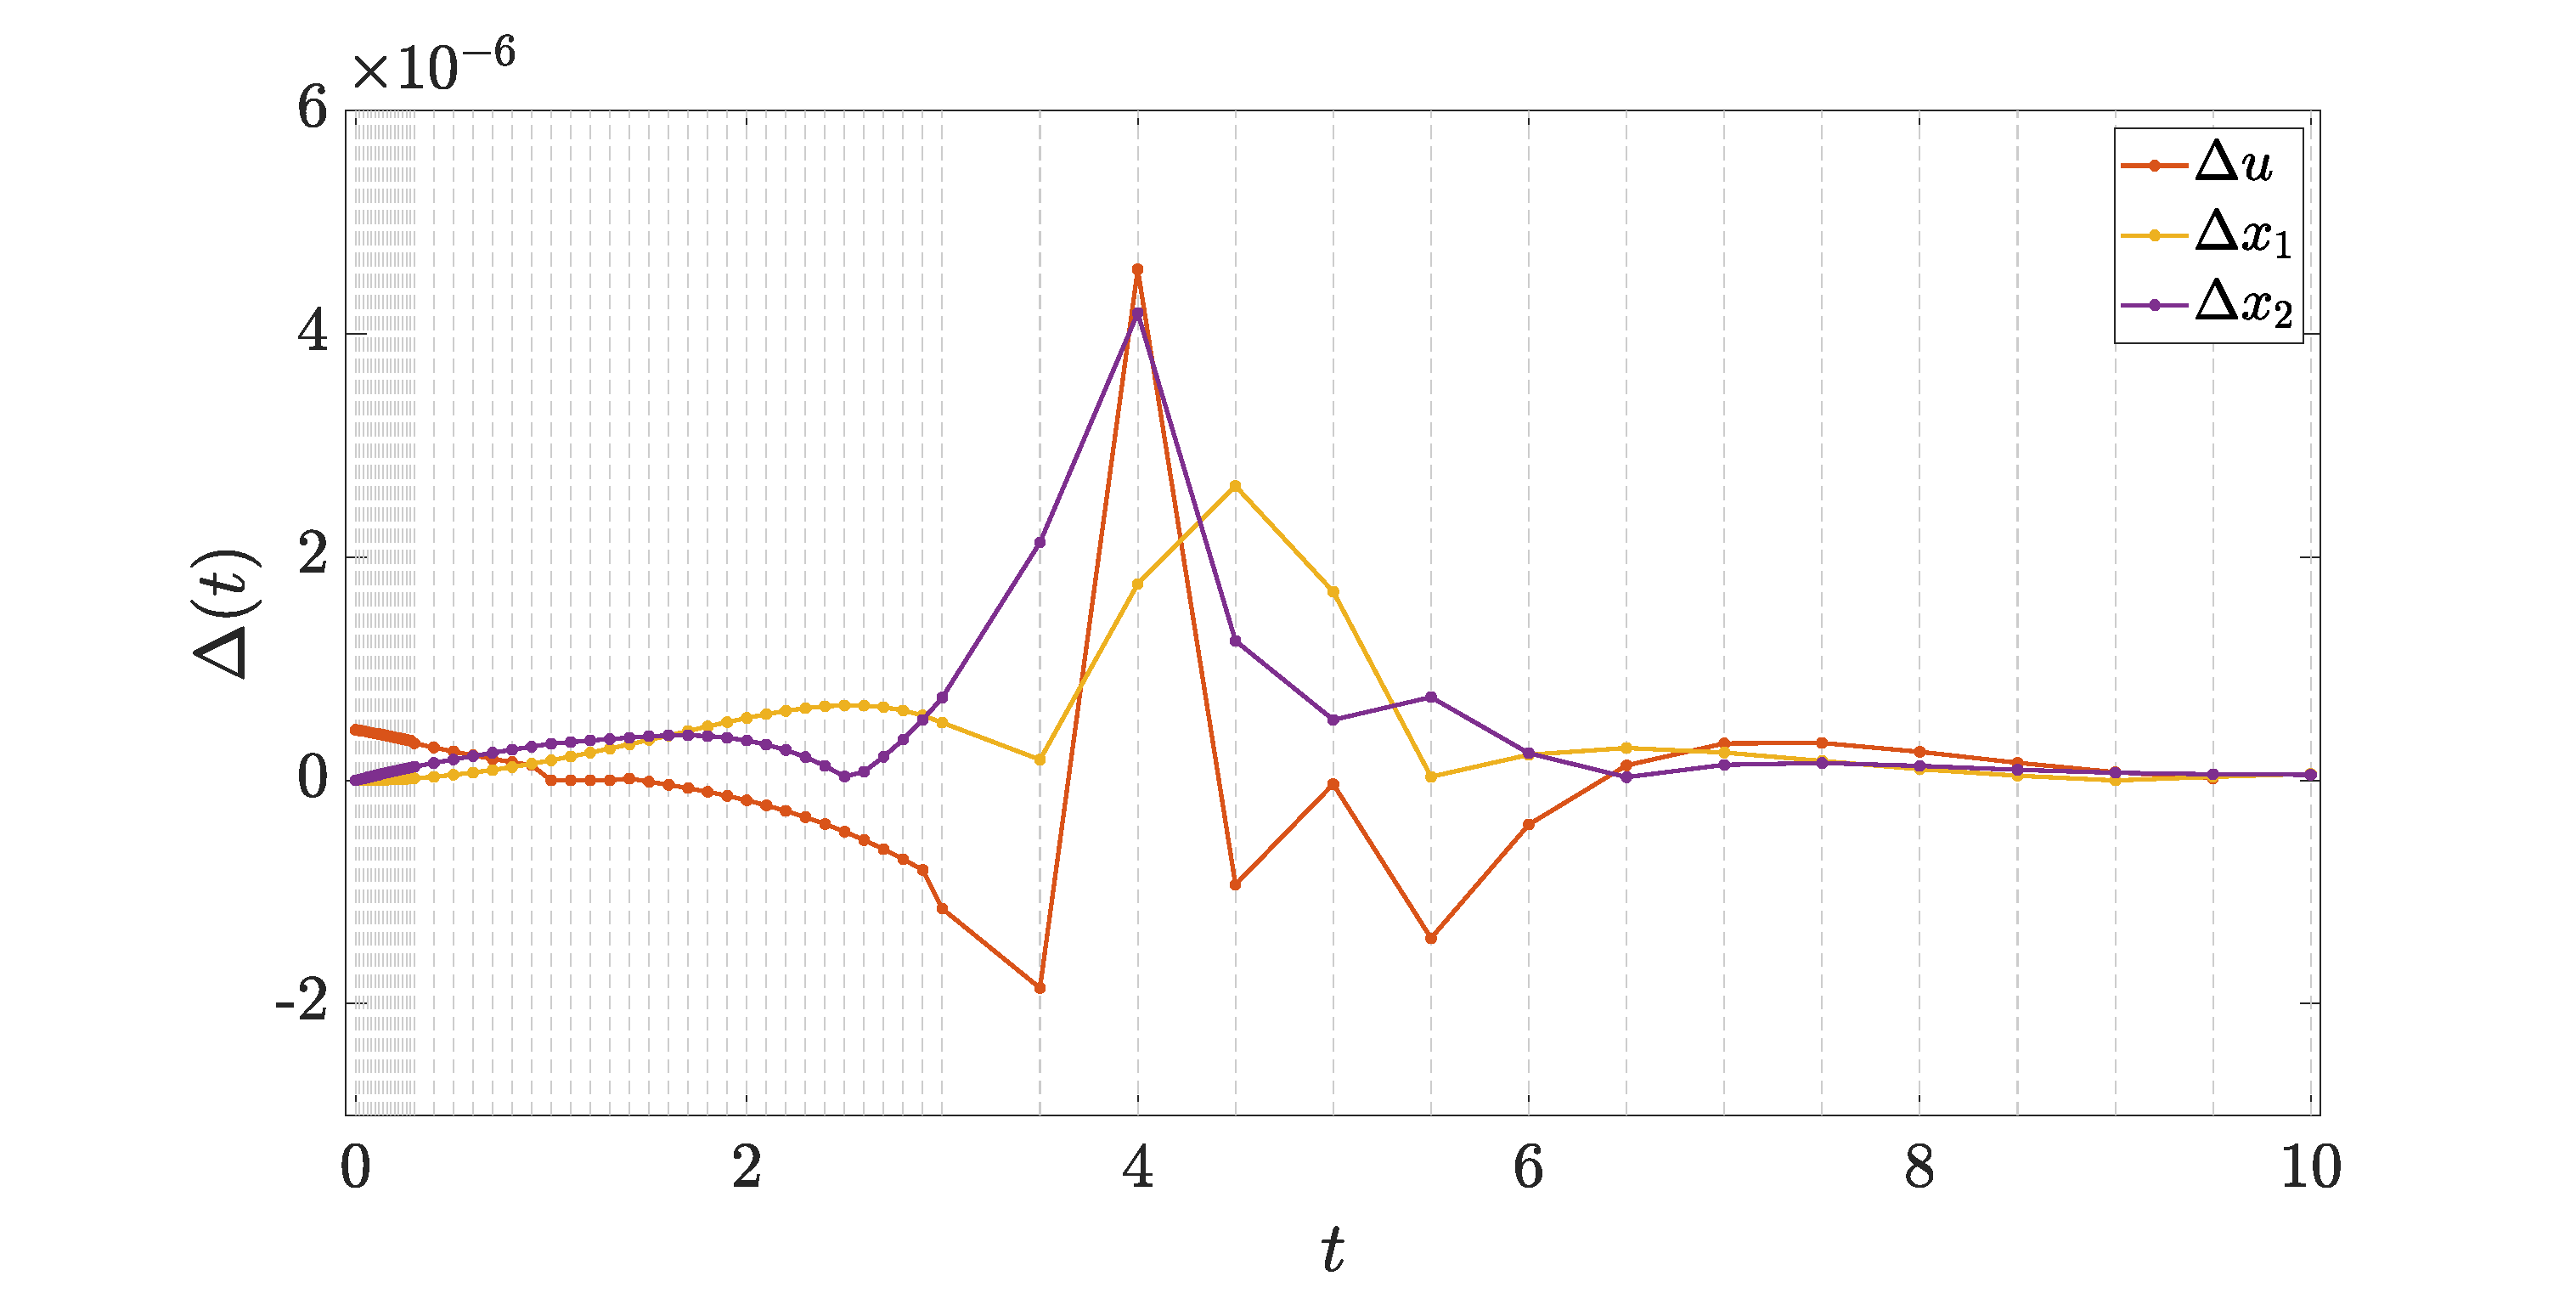
\includegraphics[trim={2cm 0.5cm 4cm 0.3cm},clip,width=1\columnwidth]{Img/delta_vanderpol}
	\caption{EXAMPLE 1: NODAL DIFFERENCES BETWEEN $\pnh$ AND $ph$ FINAL SOLUTIONS}
	\label{fig:deltavanderpol}
\end{figure}
It is worth noting that $\pnh$ method leads to an optimal solution that while respecting the given tolerance $\epsilon$, is obtained from an NLP with fewer variables than $ph$ algorithm.
Hence the final NLP obtained from $\pnh$ method required a lower computational cost and a shorter CPU time.
Furthermore considering that $ph$ and $\pnh$ have the same final mesh in terms of $S_k$ number and size, these two solution can be compared at the nodal values.
In Fig.~\ref{fig:deltavanderpol}, the difference between the $\pnh$ and $ph$ final optimal solutions, are shown.
In particular, considering that the states and the control $u$ have an order of magnitude of $10^{0}$, the two solution can be considered equal.
%%%%%%%%%%%%%%%%%%%%%%%%%%%%%%%%%%%%%%%%%%%%%%%%%%%%%%%%%%%%%%%%%%%%%%
\subsection*{Example 2: Vertical Rolling Disk}
Considering the following optimal control problem in which a vertical rolling disk has to be driven on an horizontal $x$-$y$ plane from an initial position to a final one, minimizing the control action,
\begin{subequations}\label{eq:disk}
	\begin{align}
	\underset{X \in \mathbb{R}^{6}, \, U \in \mathbb{R}^{2}}{\text{minimize}}\hspace{8mm}
	&J = \int_{0}^{T}(u_{1}^{2} +  u_{2}^{2})\,dt  \label{eq:diskcost}\\
	\text{subject to} \hspace{8mm}
	& \dot{x}_1 = \rho x_6  \cos(x_3) \hspace{10mm} t \in[0,T] \label{eq:diskdyn1}\\
	& \dot{x}_2 = \rho x_6  \sin(x_3)\hspace{10.5mm} t \in[0,T] \label{eq:diskdyn2}\\
	& \dot{x}_3 = x_5\hspace{23mm} t \in[0,T] \label{eq:diskdyn3}\\
	& \dot{x}_4 = x_6\hspace{23mm} t \in[0,T] \label{eq:diskdyn4}\\
	& \dot{x}_5 = u_1/I_{\theta}\hspace{18.2mm} t \in[0,T] \label{eq:diskdyn5}\\
	& \dot{x}_6 = u_2/(I_{\phi} + m \rho^{2})\hspace{5.8mm} t \in[0,T] \label{eq:diskdyn6}\\
	& x_6 \geq 0  \hspace{24.5mm} t \in[0,T]\\
	&X(0) = [0, 0, \pi/2, 0, 0, 0]\\	
	 x_1(T) = 10,\hspace{2mm} &x_2(T) = 10, \hspace{2mm} x_3(T) = \pi/4, \label{eq:diskfinal1}		
	\end{align}
\end{subequations}
where $T = 10$s, $m$ is the disk mass, $\rho$ is the disk radius, $I_{\theta}$ is the disk moment of inertia respect to an axis that passes through the contact point between the disk and the plane and perpendicular to the latter; $I_{\phi}$ is the disk moment of inertia respect to an axis that passes through the center of the disk and is parallel to the plane.
For what concern the states, $x_1$ and $x_2$ represent the disk trajectory on the plane, $x_3$ represents the angle between the disk rolling direction and $x$-axis on the plane and $x_4$ is the rolling angle. Instead $x_5$, $x_6$ are the steering and rolling speed, respectively.
The disk is controlled with two torques, $u_1$ for the steering action and $u_2$ for the rolling action. Starting in the plane origin ($x_1(0) = 0, \, x_2(0) = 0$) and pointing to the $y$-axis ($x_3(0) = \pi/2$) the disk has to be driven in the final position described by
Eqn.~(\ref{eq:diskfinal1}). It is worth to remember that for a more compact notation $X = [x_1, x_2, x_3, x_4, x_5, x_6]$  and $U = [u_1, u_2]$.
\begin{figure}[t]
	\centering
	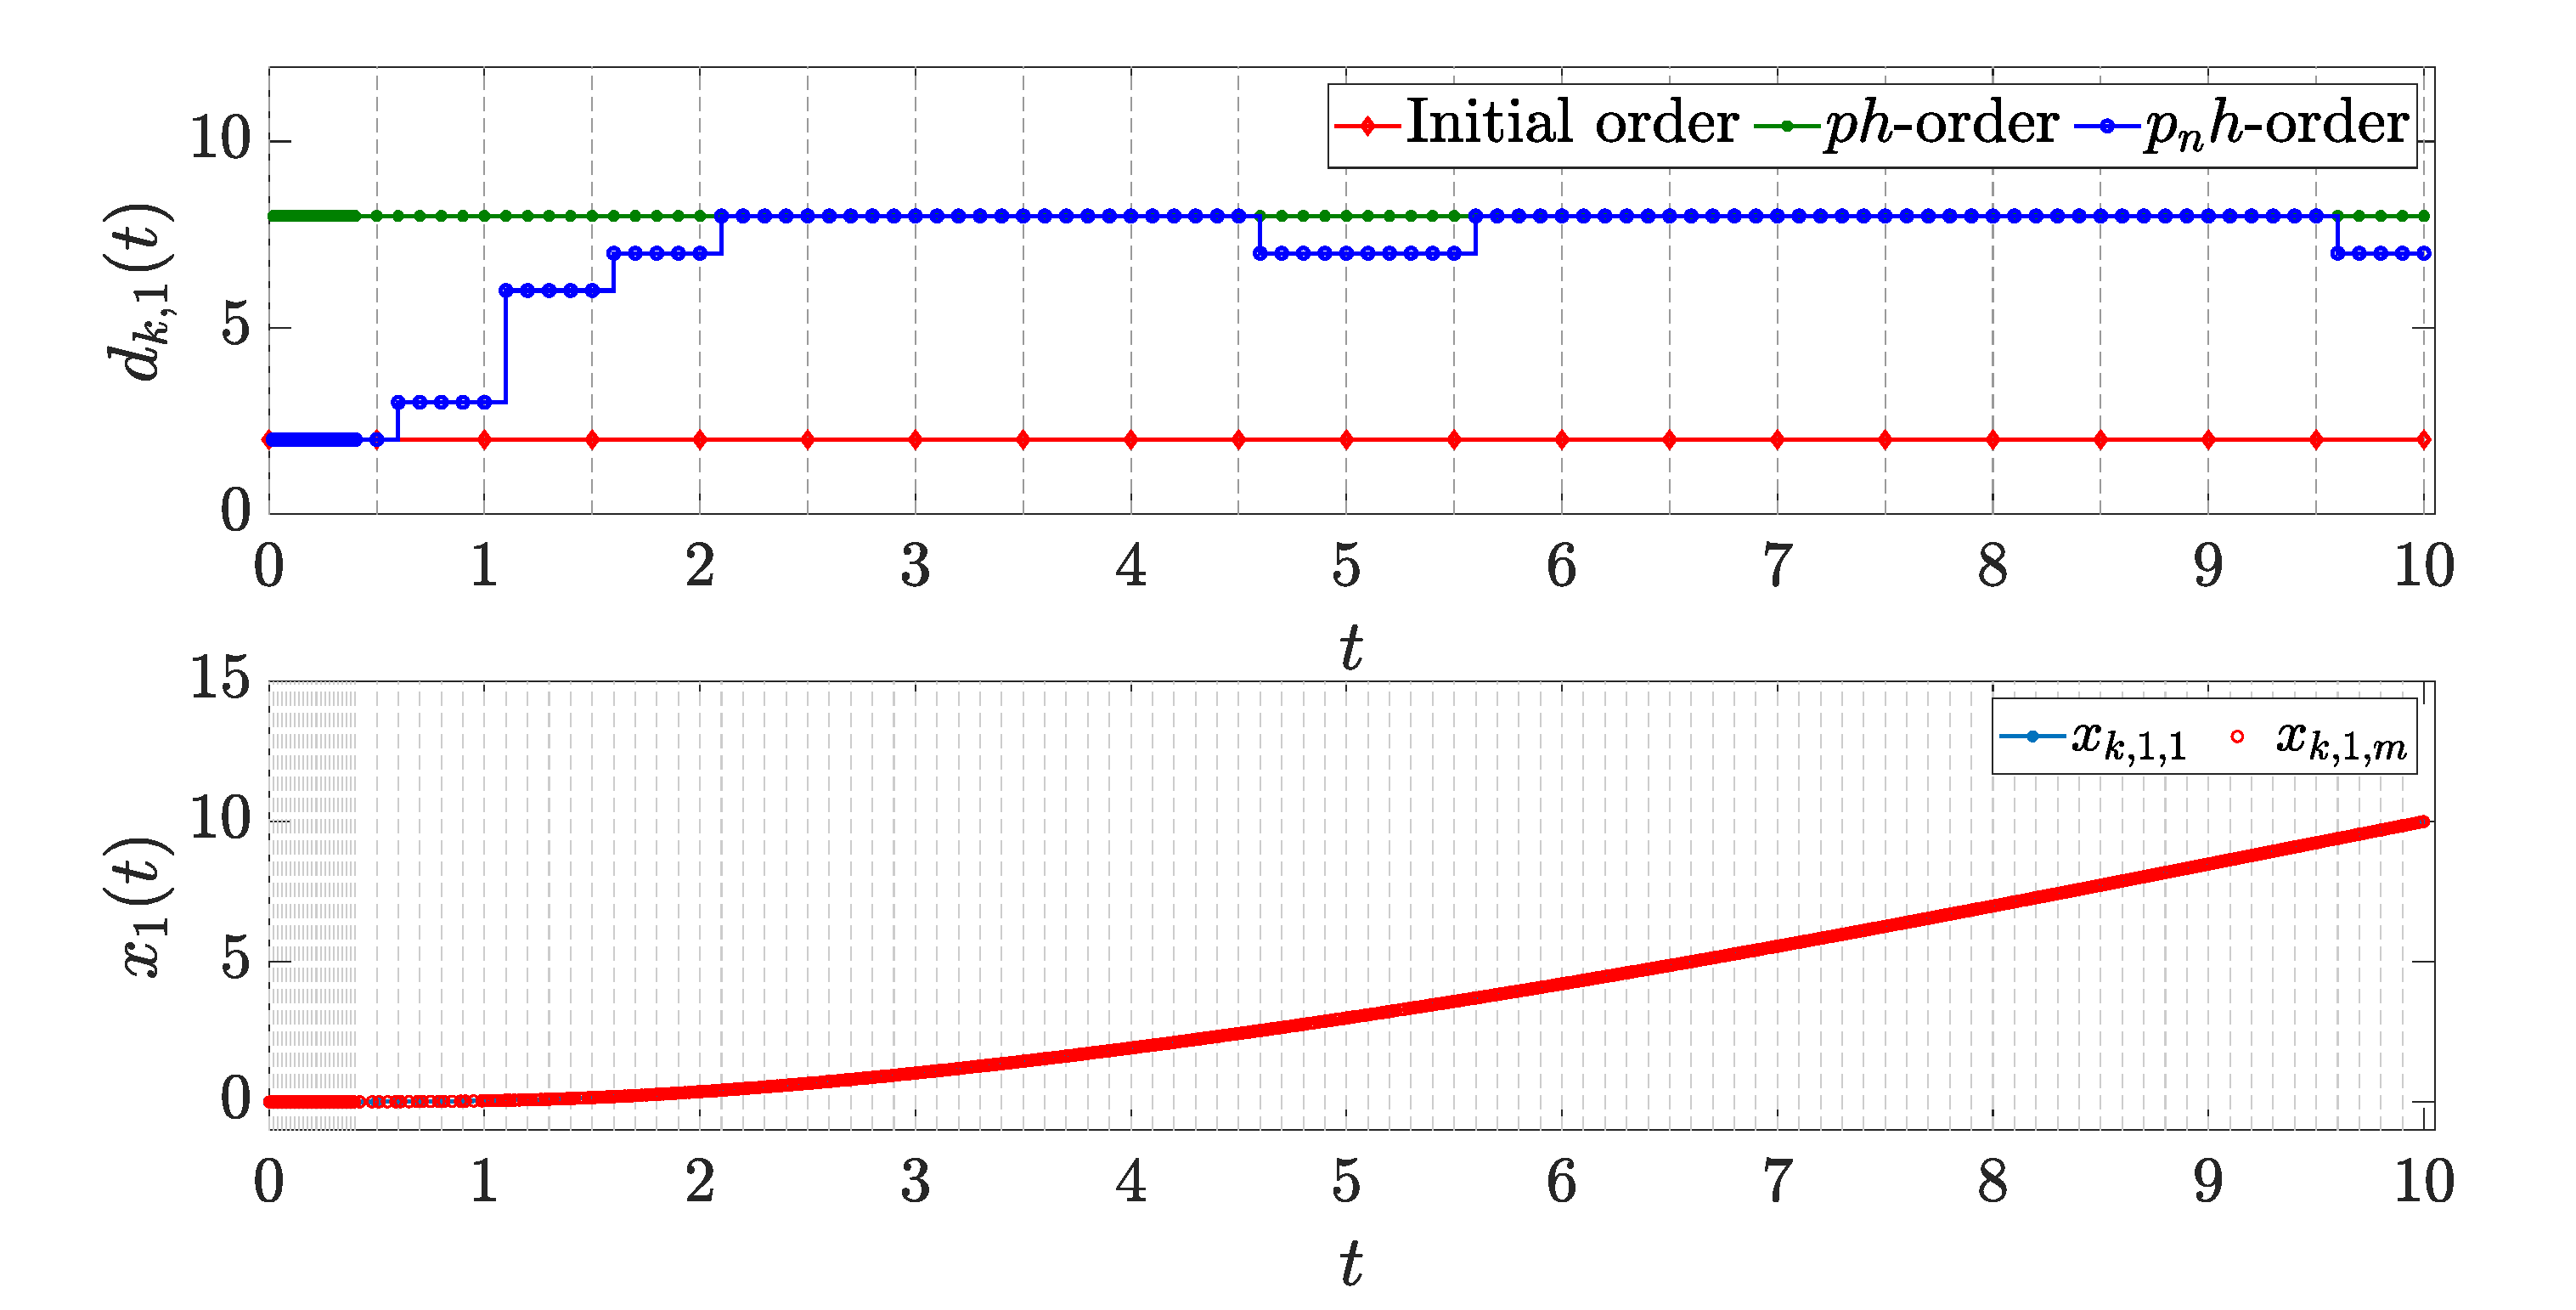
\includegraphics[trim={1cm 0.1cm 2cm 1.05cm},clip,width=1\columnwidth]{Img/pnh1_disk1}
	\caption{EXAMPLE 2: (TOP) POLYNOMIAL DEGREE OF FIRST STATE ($x_{1}$) FOR THE INITIAL MESH (RED) FOR $\pnh$ ALGORITHM (BLUE) AND FOR $ph$ ALGORITHM (GREEN), (BOTTOM)
		OPTIMAL $x_1$ PROFILE OBTAINED WITH $\pnh$.}
	\label{fig:pnh1disk}
\end{figure}
In Figs.~\ref{fig:pnh1disk}-\ref{fig:pnh2disk} (top panels) is shown, for the $\pnh$ algorithm and for the $ph$ one, the final degree of the first state component ($x_1$) and of the third one ($x_3$), respectively. Even if for some state, as for example $x_1$, the $\pnh$ and $ph$ method seem to give, for certain sector of optimal solution, the same results in terms of polynomial degree, there are other state as $x_3$ for which the two algorithm provide a very different mesh in terms of the final polynomial approximation.
In particular, the fact that the green line is always at $d_\text{max}$ means that in each mesh interval, there is at least one state that needs that polynomial order, but applying the $\pnh$ method, avoid that each state is approximated with this highest polynomial degree.
In particular, considering the solution in the range 6-9s, the state $x_1$ needs the maximum achievable order ($d_\text{max} = 8$), this leads to approximate the state $x_2$ with the same highest degree for the $ph$ method, but with a lower degree if $\pnh$ method is adopted.
Instead In Figs.~\ref{fig:pnh1disk}-\ref{fig:pnh2disk} (bottom panels) the optimal profile of $x_1$ and $x_3$ are shown. In particular, considering the gray line and the collocation points in red, it is clear where the refinement acts more.
%%%%%%%%%%%
\begin{figure}[t]
	\centering
	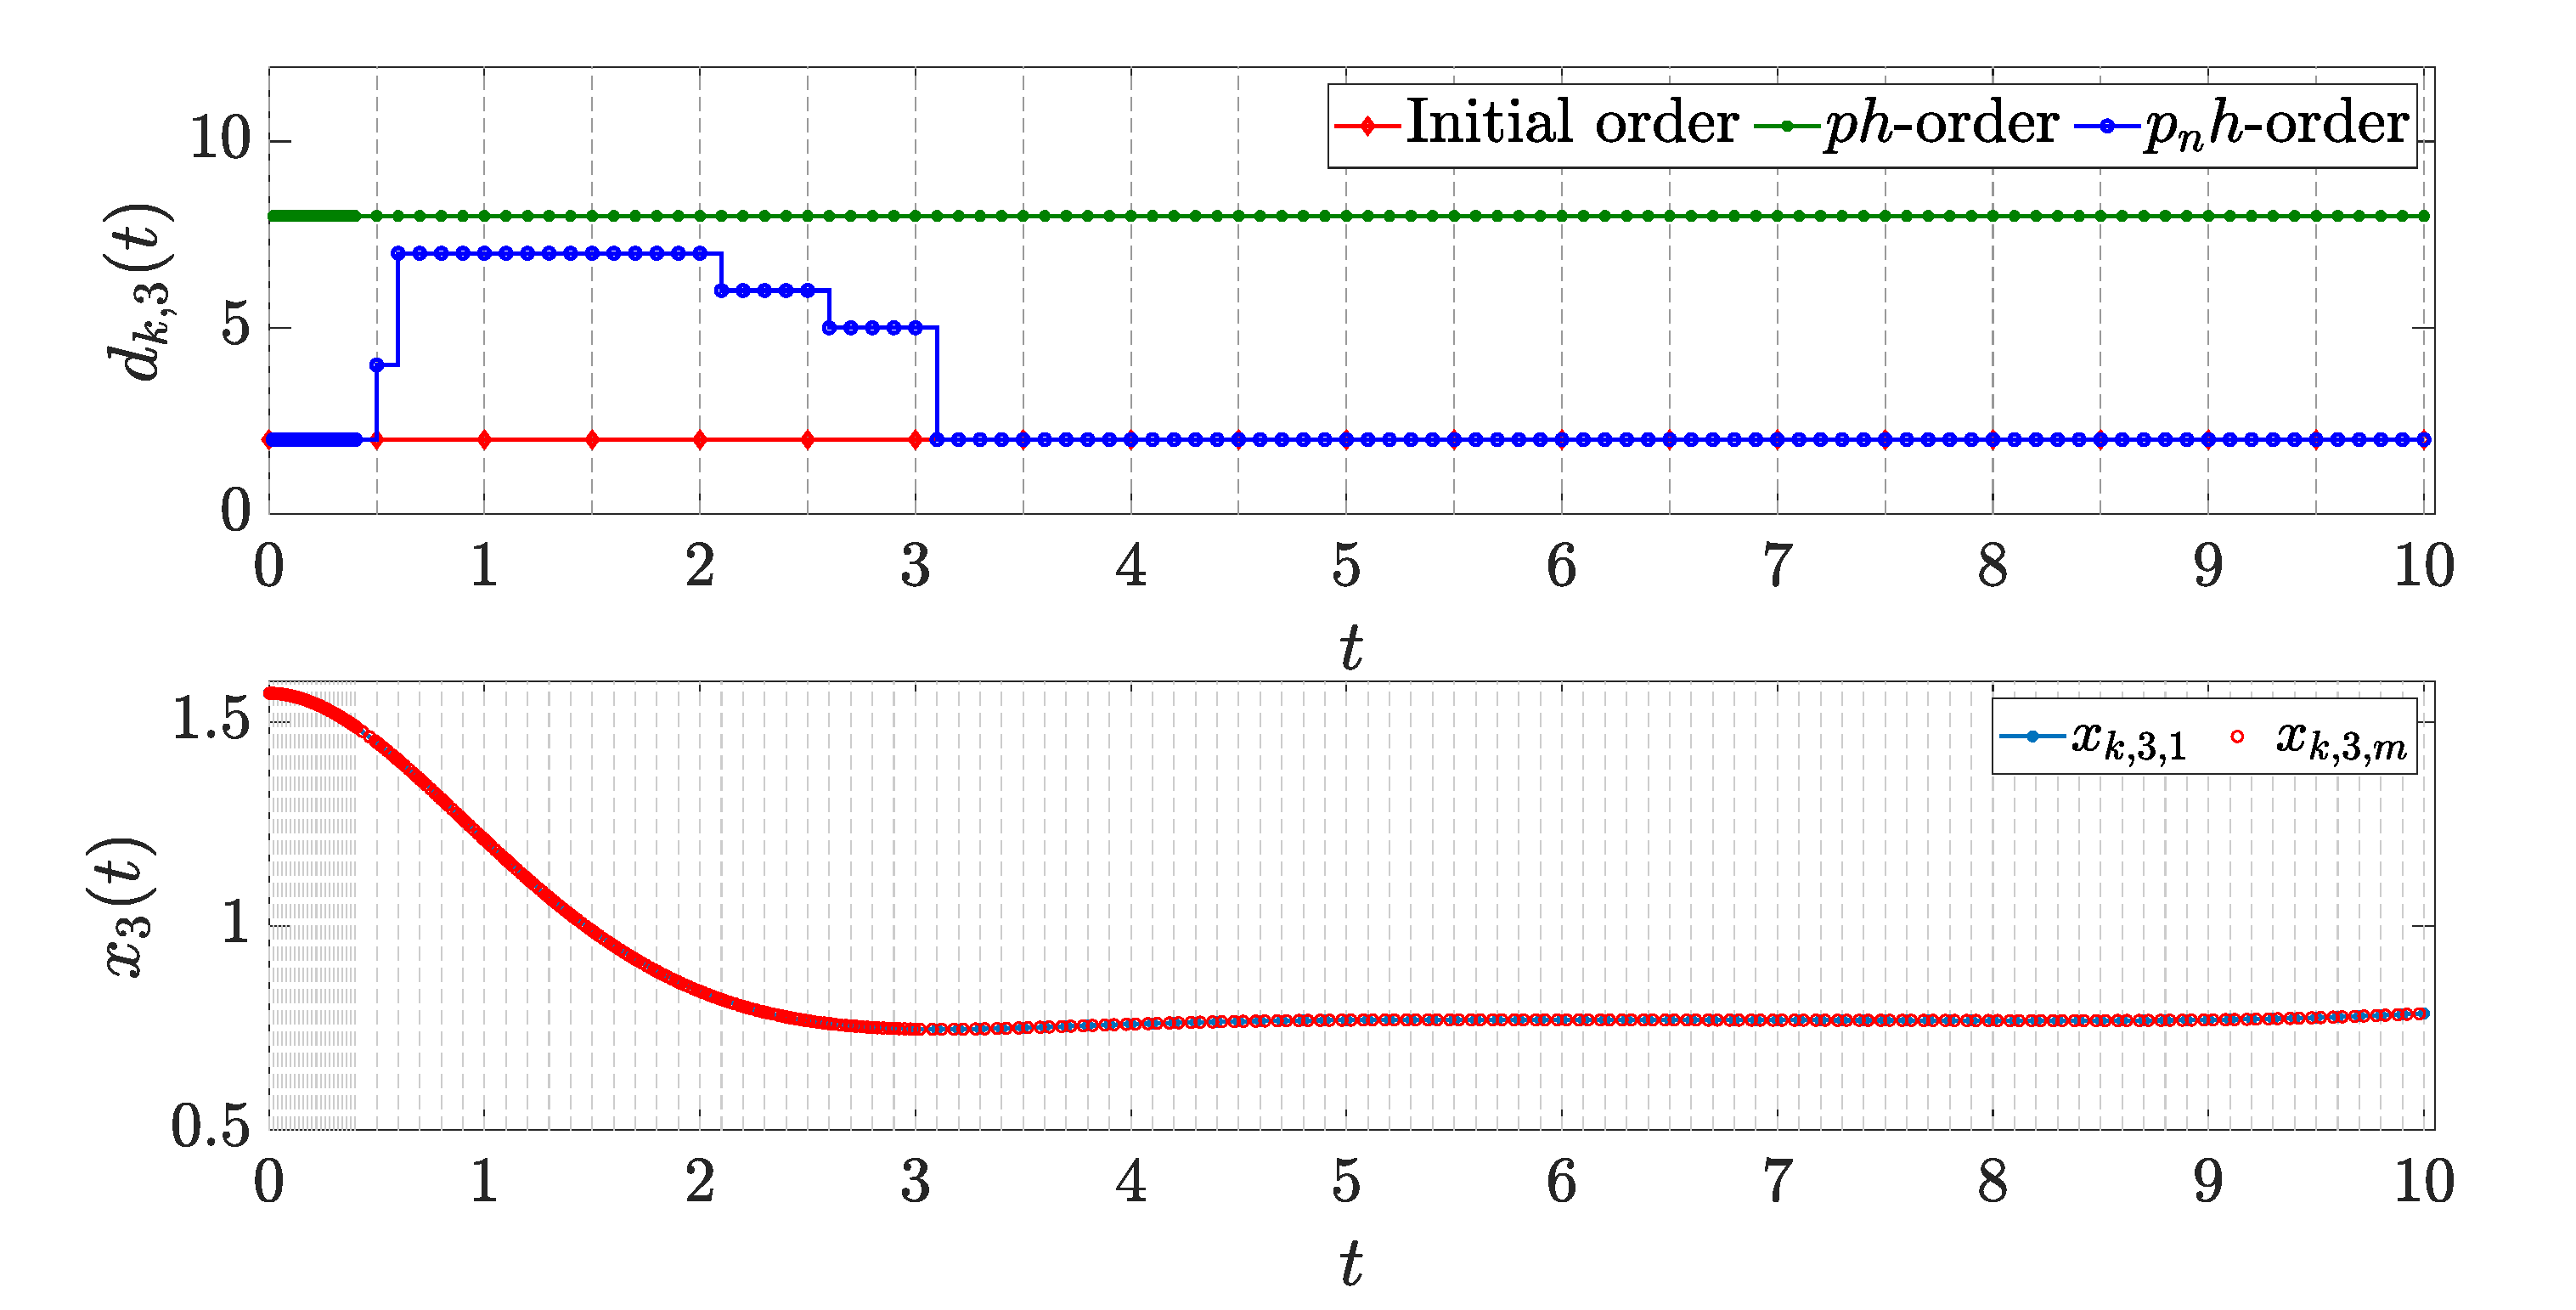
\includegraphics[trim={1cm 0.1cm 2cm 1.05cm},clip,width=1.\columnwidth]{Img/pnh2_disk2}
	\caption{EXAMPLE 2: (TOP) POLYNOMIAL DEGREE OF THIRD STATE ($x_{3}$) FOR THE INITIAL MESH (RED) FOR $\pnh$ ALGORITHM (BLUE) AND FOR $ph$ ALGORITHM (GREEN), (BOTTOM)
	OPTIMAL $x_3$ PROFILE OBTAINED WITH $\pnh$.}
	\label{fig:pnh2disk}
\end{figure}
%%%%%%%%%%%%%%
The advantages of the $\pnh$ method, respect to the $ph$ one, are shown in Tab.~\ref{tab:tabledisk}. In particular, even if $\pnh$ method needs an extra iteration, it maintains a total time equal to the $ph$ method. Furthermore, with the same $e_\text{max}$ reached, the last NLP variables of $\pnh$ are 25\% less than the original method.

For what concerns the nodal differences (obtained as the difference between te nodal value of $\pnh$ and $ph$ solutions), the maximum value is reached for $u_2$. However this difference has an order of magnitude of $10^{-6}$ which is very small considering that the control signal $u_2$ has an order of magnitude of $10^0$. Hence, the two methods lead to the same solution.
\begin{table}[t]
	\caption{EXAMPLE 2: MESH REFINEMENT RESULTS FOR THE THREE DIFFERENT TYPE OF MESH (INITIAL MESH, $ph$ FINAL MESH AND $\pnh$ FINAL MESH)}
	\begin{center}
		\label{tab:tabledisk}
		\begin{tabular}{c l l l c c c}
			& & \\ % put some space after the caption
			\hline
			\emph{Mesh} & \emph{Vars} & \emph{Sol. time} & \emph{Iter} & \emph{Tot. time} & $e_\text{max}$ \\
			\hline
			\emph{Initial} & 400 & 0.643s & / & / &  $3.6\mathrm{e}{-2}$\\
			$ph$  & 6496 & 61.62s & 4 & 287.7s & $9.8\mathrm{e}{-4}$ \\
			$\pnh$ & 4810 & 32.42s & 5 & 287.14s & $9.8\mathrm{e}{-4}$ \\
			\hline
		\end{tabular}
	\end{center}
\end{table}
%\newline
%\newline
%%%%%%%%%%%%%%%%%%%%%%%%%%%%%%%%%%%%%%%%%%%%%%%%%%%%%%%%%%%%%%%%%%%%%%
\subsection*{Example 3: Free Flying Robot}
Considering the optimal control problem of driving a free-flying robot with a propulsion system. The problem is taken from reference~\cite{Betts:book:2010}, with a modified cost function
\begin{subequations}\label{eq:free}
	\begin{align}
	\underset{X \in \mathbb{R}^{6}, \, U \in \mathbb{R}^{2}}{\text{minimize}}\hspace{8mm}
	&J = \int_{0}^{T}(u_{1}^{2} +  u_{2}^{2})\,dt  \label{eq:freecost}\\
	\text{subject to} \hspace{8mm}
	& \dot{x}_1 = x_4 \hspace{28mm} t \in[0,T] \label{eq:freedyn1}\\
	& \dot{x}_2 = x_5 \hspace{28mm} t \in[0,T] \label{eq:freedyn2}\\
	& \dot{x}_3 = x_6\hspace{28mm} t \in[0,T] \label{eq:freedyn3}\\
	& \dot{x}_4 = (u_1 + u_2)\cos(x_3)\hspace{7.5mm} t \in[0,T] \label{eq:freedyn4}\\
	& \dot{x}_5 = (u_1 + u_2)\sin(x_3)\hspace{8mm} t \in[0,T] \label{eq:freedyn5}\\
	& \dot{x}_6 = \alpha u_1 - \beta u_2\hspace{16mm} t \in[0,T] \label{eq:freedyn6}\\
	&X(0) = [-10, -10, \pi/2, 0, 0, 0]\\
	&X(T) = [0, 0, 0, 0, 0, 0] \label{eq:freefinal1}		
	\end{align}
\end{subequations}
where $x_1$ and $x_2$ are the inertial coordinates of the center of gravity, $x_3$, $x_4$ are the corresponding velocity, and $x_5$, $x_6$ are the thrust direction and the angular velocity, respectively. The thrust from two engines denoted by $u_1$ and $u_2$ serve as the control variables. Finally, $T = 12$s and $\alpha = \beta = 1$.
%%%%%%%%%%%%%
\begin{figure}[t]
	\centering
	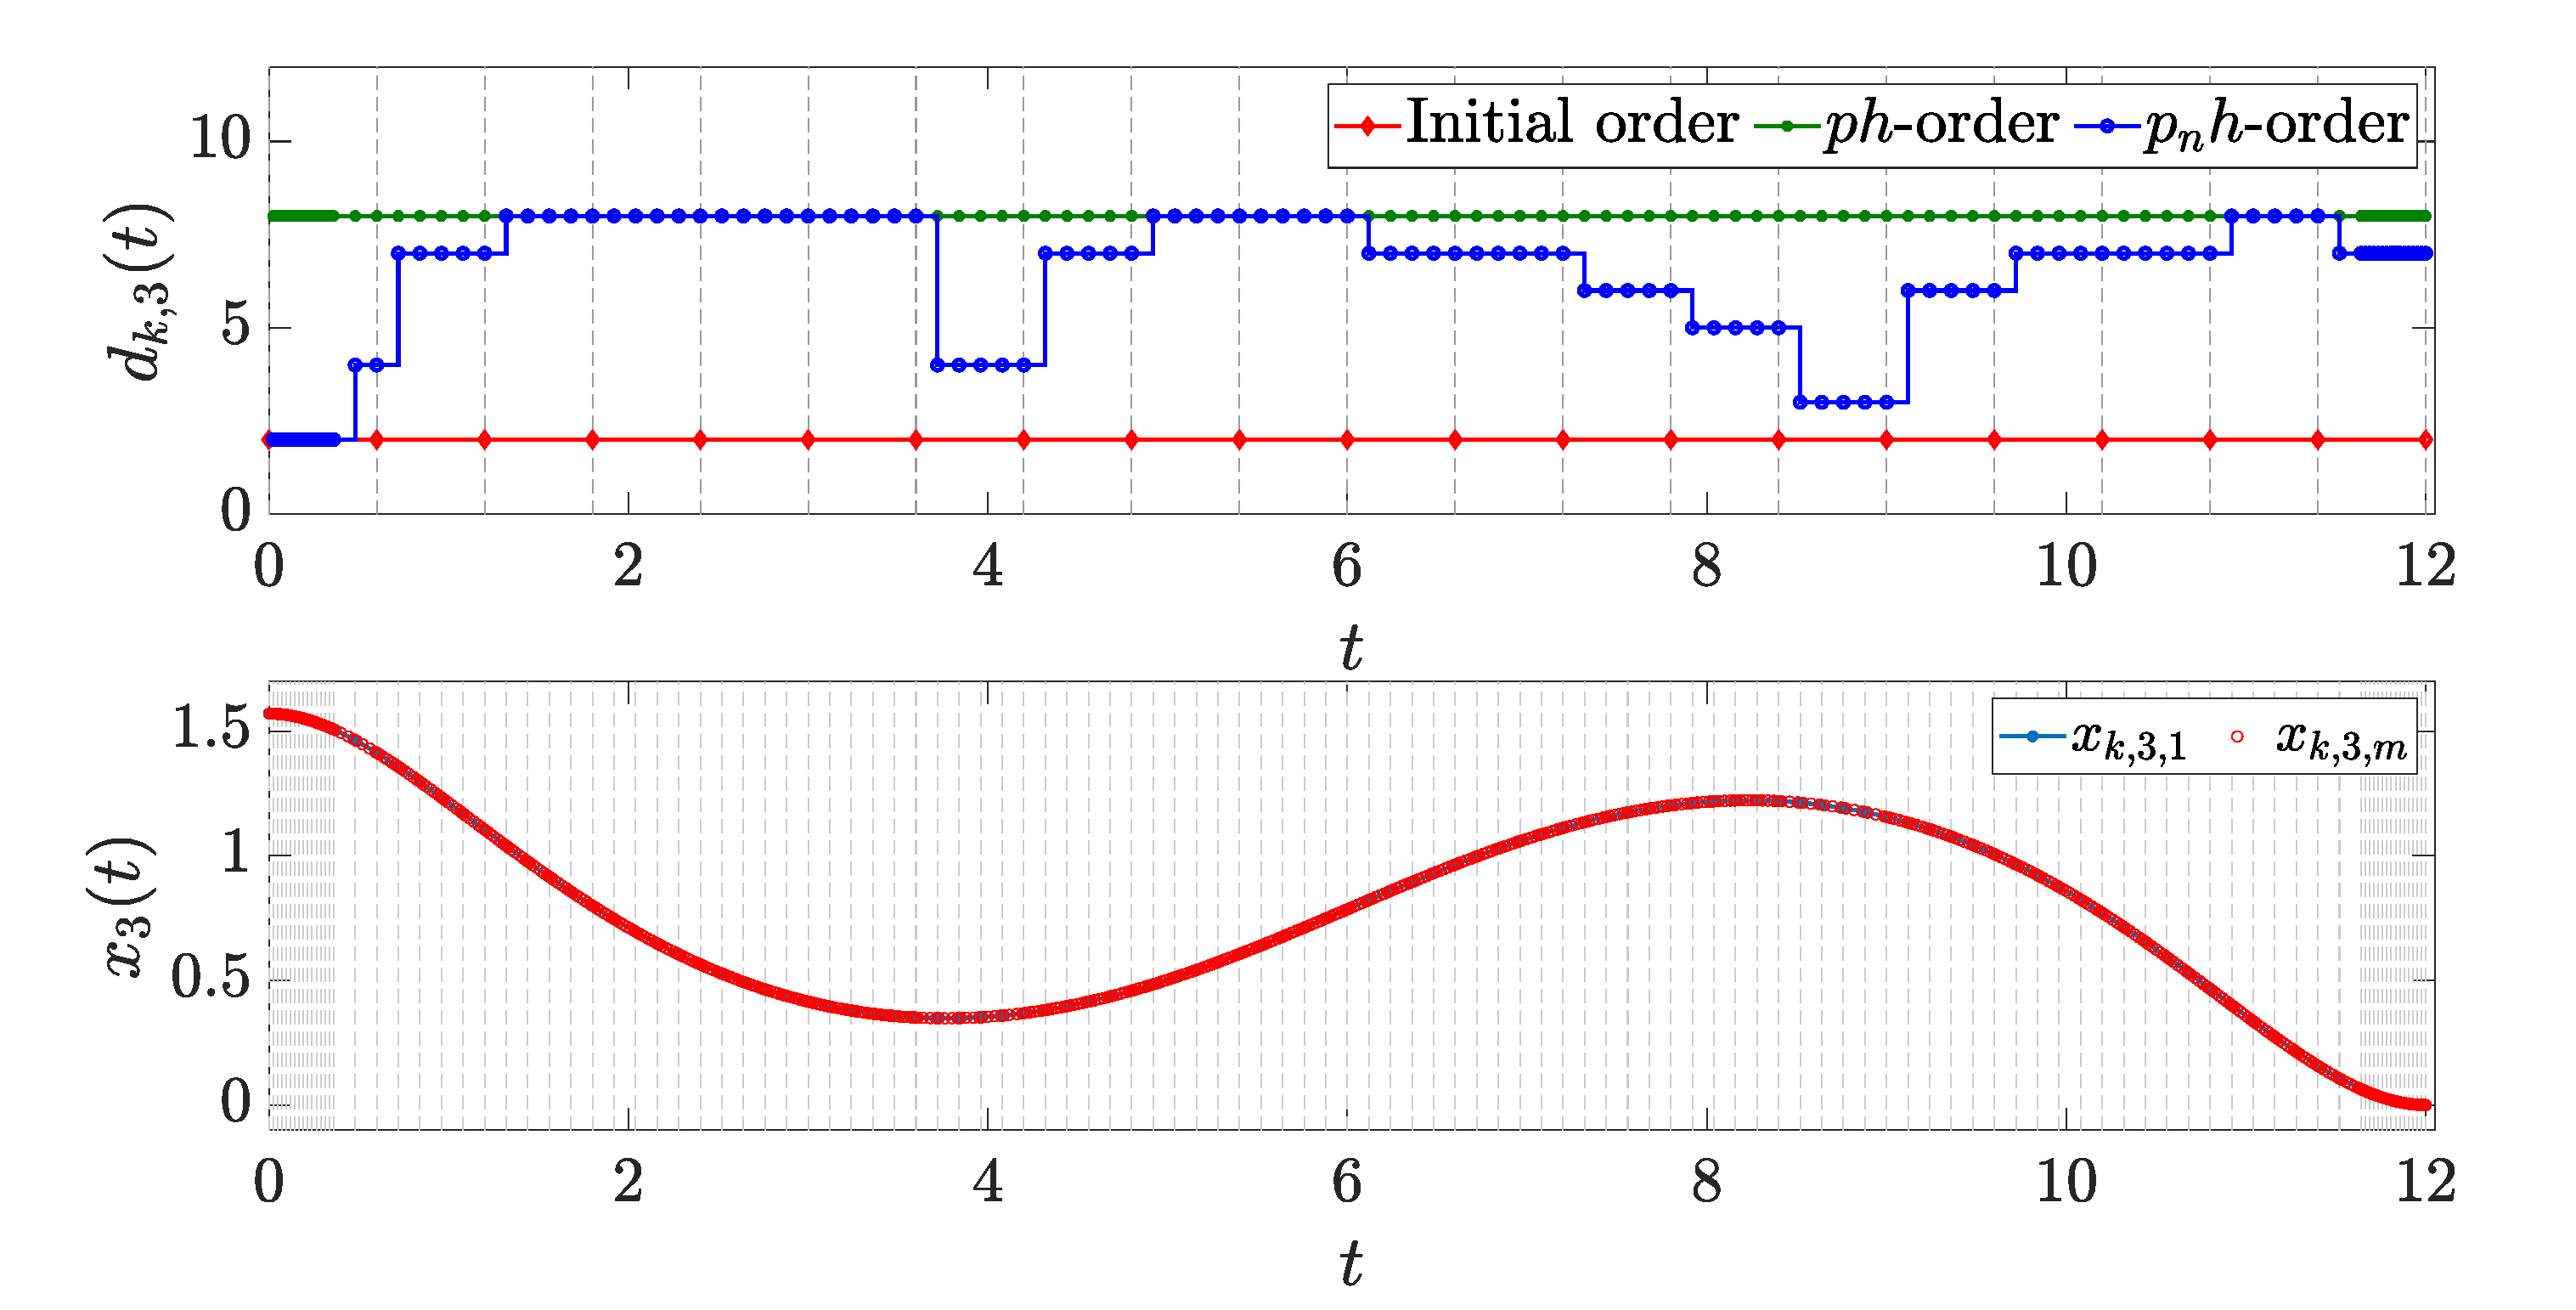
\includegraphics[trim={1cm 0.1cm 2cm 1.05cm},clip,width=1.\linewidth]{Img/pnh1_free}
	\caption{EXAMPLE 3: (TOP) POLYNOMIAL DEGREE OF $x_{3}$ FOR THE INITIAL MESH (RED), FOR $\pnh$ ALGORITHM (BLUE) AND FOR $ph$ ALGORITHM (GREEN), (BOTTOM) OPTIMAL $x_3$ PROFILE OBTAINED WITH $\pnh$. }
	\label{fig:pnh1free}
\end{figure}
%%%%%%%%%%%%%%%%
For this example,  in Fig.~\ref{fig:pnh1free}, the results for $x_3$ (hence the thrust direction) are shown. In particular, the final order required by $\pnh$ method is very different respect to the $ph$ one. Furthermore, considering the state profile, it is worth to observe that the $h$ strategy is favored at the begging and at the end of the trajectory.

The advantages of the $\pnh$ method, respect to the $ph$ one, are shown in Tab.~\ref{tab:tablefree}. In particular, the $\pnh$ method has a final $e_\text{max}$ slightly higher than the $ph$ one but guarantees $20\%$ less variables and a reduced total time.

For what concerns the nodal differences, the maximum value is reached for $x_1$. However this difference has an order of magnitude of $10^{-7}$ which is very small considering that the state $x_1$ has an order of magnitude of $10^0$. Hence, the two methods lead to the same solution.
\begin{table}[t]
	\caption{EXAMPLE 3: MESH REFINEMENT RESULTS FOR THE THREE DIFFERENT TYPE OF MESH (INITIAL MESH, $ph$ FINAL MESH AND $\pnh$ FINAL MESH)}
	\begin{center}
		\label{tab:tablefree}
		\begin{tabular}{c l l l c c c}
			& & \\ % put some space after the caption
			\hline
			\emph{Mesh} & \emph{Vars} & \emph{Sol. time} & \emph{Iter} & \emph{Tot. time} & $e_\text{max}$ \\
			\hline
			\emph{Initial} & 400 & 0.643s & / & / &  $3.7\mathrm{e}{-2}$\\
			$ph$  & 6944 & 79.75s & 4 & 367.06s & $8.9\mathrm{e}{-4}$ \\
			$\pnh$ & 5550 & 63.63s & 4 & 271.26s & $9.2\mathrm{e}{-4}$ \\
			\hline
		\end{tabular}
	\end{center}
\end{table}


%\cite{latex, goosens} 